The perceived quality of the explanations was also compared between the cold-start (Use Case 2) and post-retraining (Use Case 3) scenarios. The average scores for each explanation metric are visualized in Figure~\ref{FIG:EXP_METRICS} and shown in Table~\ref{TAB:EXP_RESULTS}.

\begin{figure}[Explanation Metrics]{FIG:EXP_METRICS}{Comparison of explanation evaluation results.}
    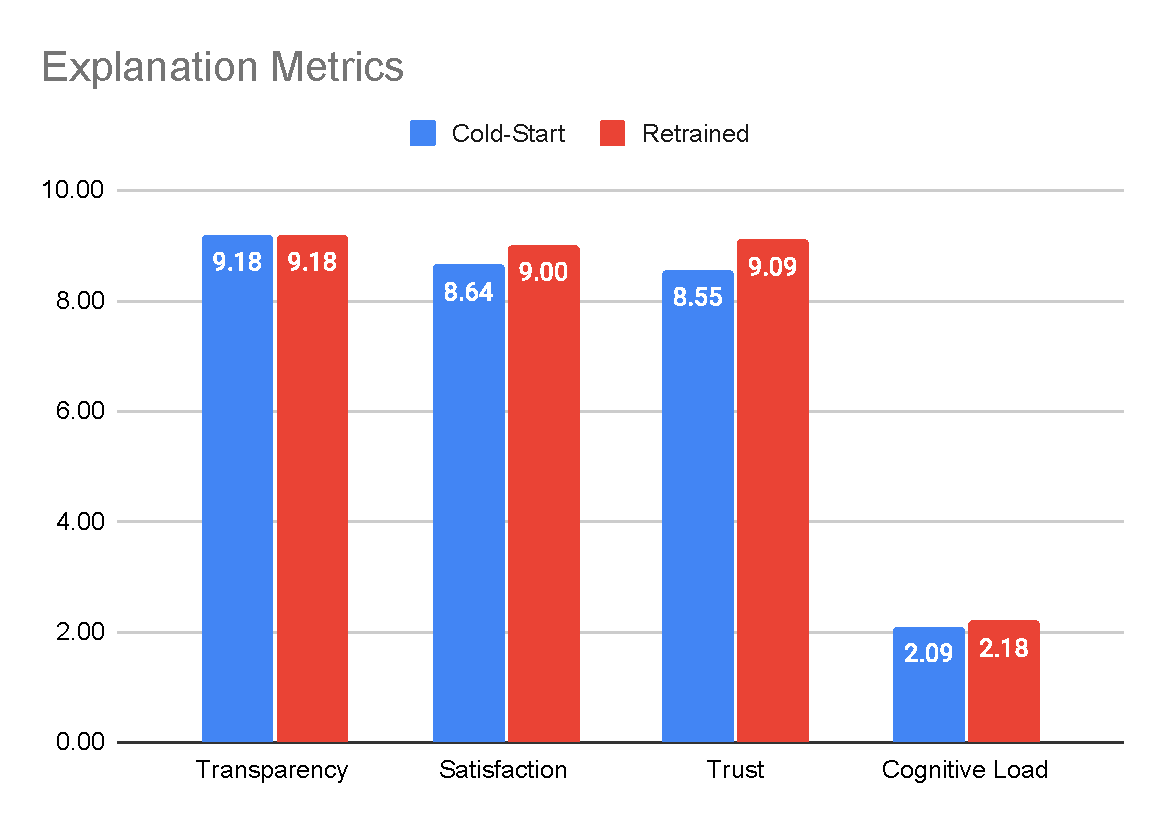
\includegraphics[width=0.8\textwidth]{exp_metrics.pdf}
\end{figure}

\begin{table}[Explanation Quality Scores]{TAB:EXP_RESULTS}{Average scores for explanation quality (1-10 scale).}
    \begin{tabular}{l c c}
        \hline
        \textbf{Metric} & \textbf{Cold-Start (UC2)} & \textbf{Retrained (UC3)} \\
        \hline
        Transparency & 9.18 & 9.18 \\
        Satisfaction & 8.64 & 9.00 \\
        Trust / Persuasiveness & 8.55 & 9.09 \\
        Cognitive Load & 2.09 & 2.18 \\
        \hline
    \end{tabular}
\end{table}

The results indicate that the explanations were rated very highly in both scenarios, particularly in terms of Transparency and low Cognitive Load. After retraining, there were observable improvements in user Satisfaction and Trust. However, a one-tailed, paired-samples t-test revealed that none of these changes were statistically significant. This suggests that while the retraining process improved the accuracy of the underlying recommendations, the graph-based method for generating explanations was perceived as consistently effective in both the cold-start and warm-start phases, with a slight increase in Satisfaction and Trust in during the latter.
